\documentclass[english]{sobraep}

\usepackage{newtxmath}
\usepackage{graphicx}

% algorithm
\usepackage[linesnumbered,ruled,vlined]{algorithm2e}
\usepackage{xcolor}
\SetKwInput{KwInput}{Input}                % Set the Input
\SetKwInput{KwOutput}{Output}              % set the Output
%%% Coloring the comment as blue
\newcommand\mycommfont[1]{\footnotesize\ttfamily\textcolor{blue}{#1}}
\SetCommentSty{mycommfont}

\newcommand{\trans}{\mathsf{T}}
\newcommand{\hermit}{\mathsf{H}}
\newcommand{\mc}[1]{\ensuremath{\mathcal{#1}}}
\newcommand{\mbb}[1]{\ensuremath{\mathbb{#1}}}
\newcommand{\Natural}{\mathbb{N}}
\newcommand{\Integer}{\mathbb{Z}}
\newcommand{\Irrational}{\mathbb{I}}
\newcommand{\Rational}{\mathbb{Q}}
\newcommand{\Real}{\mathbb{R}}
\newcommand{\Complex}{\mathbb{C}}
\newcommand{\sizecorr}[1]{\makebox[0cm]{\phantom{$\displaystyle #1$}}}

\title{SOLUTION OF NONLINEAR SISO SYSTEM THROUGH DIFFERENT PARADIGMS}


\author{Rubem Vasconcelos Pacelli$^{1}$\\
	\normalsize $^{1}$Federal University of Ceará, Forlateza -- Ceará, Brazilian\\
	\normalsize e-mail: rubem070@alu.ufc.br
}

\begin{document}

\maketitle

\begin{abstract}
	This paper shows different methods for solving a nonlinear regression problem. The same dataset with 250 observations of a nonlinear SISO (single input, single output) system is used for the following methods: least-squares regressor by parts, $k$th order polynomial regressor, Mamdani fuzzy system, and 0-order Takagi-Sugeno fuzzy system. All models are analyzed via $R^2$ for different hyperparameters (polynomial order, number of intervals, etc...). The best solutions' residues and scatter plots are analyzed and discussed.
\end{abstract}

\begin{keywords}
	Nonlinear regression problem, Mamdani fuzzy system, Takagi-Sugeno fuzzy system, polynomial regressor, regression by parts. 
\end{keywords}

% \let\thefootnote\relax\footnotetext{\hspace*{-5mm}This footnote will be used only by the Editor and Associate Editors.~The edition in this area is not permitted to the authors. This footnote must not be removed while editing the manuscript.}

% \section*{NOMENCLATURE}

% \symbolnomenclature{$P$}{Number of poles.}
% \symbolnomenclature{$V_{qd}$}{Stator voltage \textit{dq} components.}
% \symbolnomenclature{$I_{qd}$}{Stator current \textit{dq} components.}	

%~~~~~~~~~~~~~~~~~~~~~~~~~~~~~~~~~~~~~~~~
%Sections
%~~~~~~~~~~~~~~~~~~~~~~~~~~~~~~~~~~~~~~~~

%Introduction

\section{Least-Squares by parts}

The Lest-Squares (LS) method is an approximation technique for overdetermined systems that aims to minimize the squared value of the residuals. Such systems are characterized by having more equations than variables and are easily found in practice \cite{kay1993fundamentals}.

Consider the example of a discrete-time SISO system, where $x_n, y_n \in \mathbb{R}$ are, respectively, their input and output values at the instant $n \in \left\{1,2,...,N\right\}$. At each instant, one has an equation where the input and output are related through a set of \(K+1\) parameters, $\boldsymbol{\thetaup} \in \mathbb{R}^{K+1}$. Mathematically, one can define the output variable as
\begin{align}
    y_n = f(x_n;\boldsymbol{\thetaup})
\end{align}

When $f(\cdot)$ is a linear function, the LS problem is commonly called Ordinary Least-Square (OLS). The least-squares method aims to minimize the following cost function
\begin{align}
    J\left( \hat{\boldsymbol{\thetaup}} \right) = \sum_{n=1}^{N} e_n^2,
\end{align}
where \(\hat{y}_n\) and \(\hat{\boldsymbol{\thetaup}}\) are the estimates of \(y_n\) and \(\boldsymbol{\thetaup}\), respectively, and \(e_n = y_n - \hat{y}_n\) is the residual signal. Although the OLS method has no optimality associated with it, various practical problems, such as regression analysis, can be solved via OLS since no probabilistic assumptions need to be made about the data \cite{kay1993fundamentals}.

The linear regressor output of the SISO system can be expressed as
\begin{align}
    \label{eq:y_n}
    \hat{y}_n = f(x_n;\hat{\boldsymbol{\thetaup}}) = \hat{a}x_n + \hat{b},
\end{align}

where \(\hat{\boldsymbol{\thetaup}} = \begin{bmatrix} \hat{a} & \hat{b} \end{bmatrix}^\trans\). By using the Equation \eqref{eq:y_n}, we can rewrite te cost function as
\begin{align}
    \label{eq:J}
    J\left( \hat{\boldsymbol{\thetaup}} \right) = \sum_{n=1}^{N} \left( y_n - \hat{a}x - \hat{b} \right)^2.
\end{align}
The Equation \eqref{eq:J} describes a convex function whose surface is a hyperparaboloid. The minimum value of the cost function corresponds to the set of coefficients sought \cite{diniz1997adaptive}. In other words, we can state that
\begin{align}
    \exists \;\; \hat{\boldsymbol{\thetaup}}^{\star} \in \mathbb{R}^{K+1} \mid J\left(\hat{\boldsymbol{\thetaup}}^{\star}\right) < J\left(\hat{\boldsymbol{\thetaup}}\right) \;\; \forall \;\; \hat{\boldsymbol{\thetaup}} \neq \hat{\boldsymbol{\thetaup}}^{\star}
\end{align}

By calculating the derivative of \(J\left( \hat{\boldsymbol{\thetaup}} \right)\) with respect to \(\hat{a}\) and \(\hat{b}\), we get
\begin{align}
    \frac{\partial J\left( \hat{\boldsymbol{\thetaup}} \right)}{\partial \hat{a}} = -2 \sum_{n=1}^{N} x_n\left( \hat{y}_n - \hat{a}x_n - \hat{b} \right) = 0
\end{align}
and
\begin{align}
    \frac{\partial J\left( \hat{\boldsymbol{\thetaup}} \right)}{\partial \hat{b}} = -2 \sum_{n=1}^{N} \left( \hat{y}_n - \hat{a}x_n - \hat{b} \right) = 0,
\end{align}
respectively. The solution of this system of equations is given by
\begin{align}
    \hat{a} = \frac{\hat{\sigma}_{xy}}{\hat{\sigma}^2_x}
\end{align}
and
\begin{align}
\hat{b} = \hat{\mu}_y - \hat{a}\hat{\mu}_x,
\end{align}
where \(\hat{\mu}_{\cdot}\) and \(\hat{\sigma}_{\cdot}^2\) are the sample mean and sample variance with respect to its subscript, respectively, and \(\hat{\sigma}_{xy}\) is the estimate of the covariance of \(x_n\) and \(y_n\).

Although the solution of the SISO OLS method is rather straightforward, many input-output relationships found in practice have nonlinearities. In these cases, one can resort to applying a transformation to the data in order to linearize the problem. Another approach is to utilize the OLS method in intervals where the scatter plot behaves approximately linear, yielding a set of linear curves with their respective parameters for each path. It is also possible to exploit other nonlinear regression methods, such as polynomial regression. The scatter plot of the dataset, shown in Figure \ref{fig:scatterplot}, suggests that the input-output relationship is severely nonlinear. Nonetheless, there are intervals where the function can be approximated to a linear curve. A natural hyperparameter arises in this approach: the number of intervals considered. The main trade-off is that the more intervals considered, the better the performance of the coefficient of determination tends to be. However, more parameters are needed to characterize the curve. The best solution is to solve the nonlinear problem with as few parameters as possible.

\begin{figure}[H]
	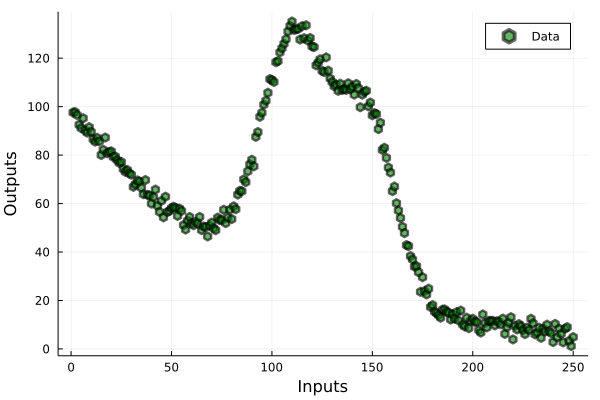
\includegraphics[scale=.37]{../figs/OLS-by-parts/scatterplot.png}
	\centering
	\caption{Scatter plot of the dataset.}
	\label{fig:scatterplot}
\end{figure}

In this paper, the OLS algorithm by parts is implemented for different sets of curve intervals, \(\left\{ R_i \right\}_{i=1}^{I}\), where \(I \in \left\{ 4,5,6 \right\}\) and \(R_i\) is the \(i\)th interval. Since it is obtained a coefficient of determination, \(R^2\), for each interval, the mean, \(\mu_{R^2}\), and the variance, \(\sigma_{R^2}^2\), is analyzed for each configuration. The Figure \ref{fig:OLS-by-parts} shows where the delimiters have been placed, in addition to the linear curves obtained by the OLS algorithm. The Algorithm \ref{alg:OLS-by-parts} summarizes the behavior of the OLS algorithm by parts, and the Table \ref{tab:OLS-performance} shows the performance for each value of \(I\).

\begin{figure}[htp]
    \subfloat[\centering\(I=4\)]{%
    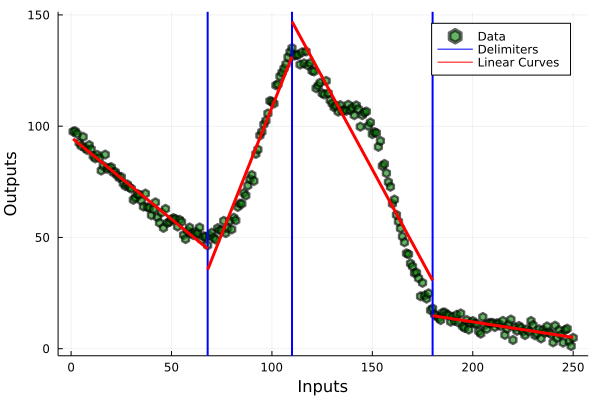
\includegraphics[clip,width=\columnwidth]{../figs/OLS-by-parts/OLS_by_4parts.png}%
    }
    
    \subfloat[\centering\(I=5\)]{%
    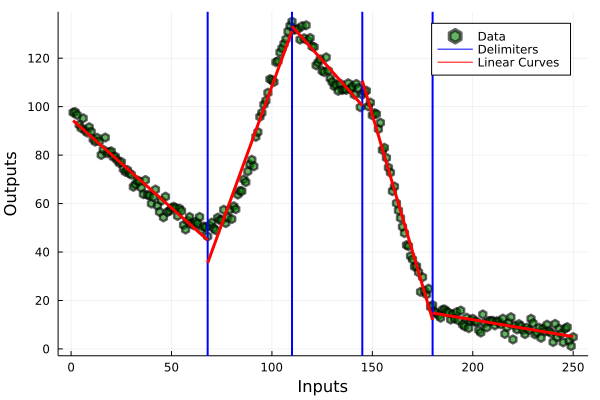
\includegraphics[clip,width=\columnwidth]{../figs/OLS-by-parts/OLS_by_5parts.png}%
    \label{fig:OLS-by-parts-I5}
    }

    \subfloat[\centering\(I=6\)]{%
    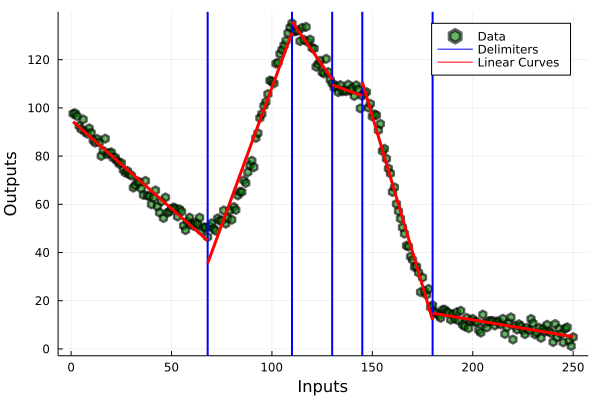
\includegraphics[clip,width=\columnwidth]{../figs/OLS-by-parts/OLS_by_6parts.png}%
    \label{fig:OLS-by-parts-I6}
    }
    
    \caption{The OLS method by parts.}
    \label{fig:OLS-by-parts}
\end{figure}

\begin{algorithm}[!ht]
    \DontPrintSemicolon
      
      \KwInput{\(\left\{ (x_n, y_n) \right\}_{n=1}^N\)}
    %   \KwOutput{\(\left\{ \left( \hat{a},\hat{b} \right), R^2 \right\}_{i=1}^I\)}
    %   \KwData{Testing set $x$}
    %   $\sum_{i=1}^{\infty} := 0$ \tcp*{this is a comment}
    %   \tcc{Now this is an if...else conditional loop}
      \For{\(I\in \left\{ 4,5,6 \right\}\)}
        {
            % Do something    \tcp*{this is another comment}
            \For{\(i \in \left\{ 1,2, ... I \right\}\)}{
                \For{\((x_n, y_n) \in R_i\)}{
                    \(N_i \leftarrow\) number of samples that belongs to \(R_i\)

                    \(\hat{\mu}_x \leftarrow \frac{1}{N_{i}}\sum x_n\)

                    \(\hat{\mu}_y \leftarrow \frac{1}{N_{i}}\sum y_n\)
                    
                    \(\hat{\sigma}_{xy} \leftarrow \frac{1}{N_{i}}\sum x_ny_n - \hat{\mu}_x\hat{\mu}_y\)
                    
                    \(\hat{\sigma}_{x}^2 \leftarrow \frac{1}{N_{i}}\sum x_n^2 - \hat{\mu}_x^2\)
                    
                    \(\hat{a} \leftarrow \frac{\hat{\sigma}_{xy}}{\hat{\sigma}_{x}^2} \)

                    \(\hat{b} \leftarrow \hat{\mu}_y - \hat{a}\hat{\mu}_x\)
                }
            }
        }
    
    \caption{OLS algorithm by parts}
    \label{alg:OLS-by-parts}
\end{algorithm}

\begin{table}[H]
	\centering
	\caption{OLS by parts performance - \(R^2\)}
	\footnotesize
	\setlength{\tabcolsep}{5pt}
	\begin{tabular}{ccccccccc}
		% \toprule [1.3pt]	
		% \multicolumn{4}{c}{ \textbf{Style} } \\
		\hline
		\multirow{2}{*}{\(I\)} & \multirow{2}{*}{\(i=1\)} & \multirow{2}{*}{\(i=2\)} & \multirow{2}{*}{\(i=3\)} & \multirow{2}{*}{\(i=4\)} & \multirow{2}{*}{\(i=5\)} & \multirow{2}{*}{\(i=6\)} & \multirow{2}{*}{\(\mu_{R^2}\)} & \multirow{2}{*}{\(\sigma_{R^2}^2\)} \\
		&  &  & \\		
		\hline
		4 & 0.962 & 0.952 & 0.911 & 0.627 & NaN & NaN & 0.863 & 0.018 \\
        \hline
		\textbf{5} &  \textbf{0.962}  & \textbf{0.952} & \textbf{0.895} & \textbf{0.985} & \textbf{0.627} & \textbf{NaN} & \textbf{0.884} & \textbf{0.017} \\
		\hline
		6 & 0.962 & 0.952 & 0.876 & 0.314 & 0.985 & 0.627 & 0.786 & 0.059 \\
		\hline
	\end{tabular} \label{tab:OLS-performance}
\end{table}

The best solution is found for \(I=5\), highlighted in the Table \ref{tab:OLS-performance}. Although it is expected to achieve better performance as it is increased the number of intervals, it is possible to notice by the Figure \ref{fig:OLS-by-parts-I6} that the placement of the delimiters does not contribute for a good linear approximation (there are outliers for \(i=4\)). This fact decreases \(R^2\) and makes it worse when compared with the case where \(I=5\).

In addition to the regressor performance, one can analyze the distribution of the residuals. Let \(\xi_n\) be the normalized residual value, that is, \(\xi_n = e_n/\sigma_e\). For a good placement of the intervals, the normalized residual distribution approximates to a zero-mean Gaussian distribution with unitary variance, i.e., \(\xi_n \sim N(0, 1)\). The Figure \ref{fig:distribution} shows the distribution (for \(i=1\)) of the residuals along with the Gaussian distribution \cite{leon1994probability}.

\begin{figure}
    \centering
    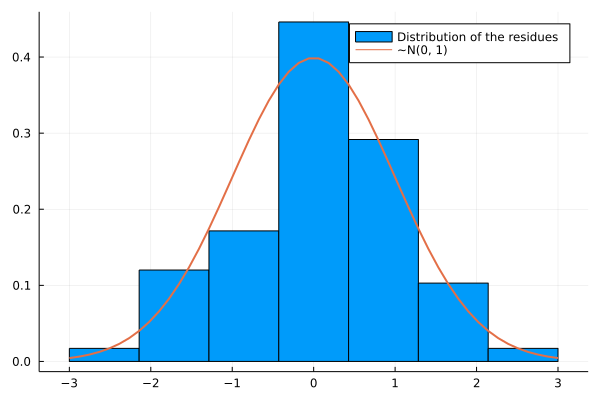
\includegraphics[scale=0.35]{../figs/OLS-by-parts/residues_PDF_I5i1.png}
    \caption{Distribution of the residuals.}
    \label{fig:distribution}
\end{figure}

\section{Polynomial Regression}

The Polynomial regression is a nonlinear method which extends the concept of the SISO OLS algorithm. At the instant \(n\), the input \(x_n\) is utilized to generate the tuple \(\left( h_{n,1}, h_{n,2}, ..., h_{n,K} \right)\), where \(h_{n,k}=x_n^k,\;\forall\; k \in \left\{ 1, 2, ..., K \right\}\). Therefore, the SISO model is transformed into a MISO (Multiple Input, Single Output) model, where the \(k\)th input of the \(n\)th instant is \(x_n\) to the power \(k\). Note that, albeit this model is not linear with relation to \(x_n\), it is with relation to \(h_{n,k}\), that is,
\begin{align}
    y_n & = f(x_n;\hat{\boldsymbol{\thetaup}}) = \mathbf{h}_n^\trans \hat{\boldsymbol{\thetaup}} \nonumber \\
    & = \hat{\theta}_0 + \hat{\theta}_1 h_{n,1} + \hat{\theta}_2 h_{n,2}  + \cdots + \hat{\theta}_K h_{n,K},
\end{align}
where \(\hat{\boldsymbol{\thetaup}} = \begin{bmatrix}
    \hat{\theta}_0 & \hat{\theta}_0 & \cdots & \hat{\theta}_K
\end{bmatrix}^\trans \in \mathbb{R}^{K+1}\) and \(\mathbf{h}_n = \begin{bmatrix}
    1 & h_{n,1} & h_{n,2} & \cdots & h_{n,K}
\end{bmatrix}^\trans  \in \mathbb{R}^{K+1}\). The matricial notation for all \(N\) observations is given by
\begin{align}
    \hat{\mathbf{y}} = \mathbf{H} \hat{\boldsymbol{\thetaup}}
\end{align}
where \(\mathbf{y} = \begin{bmatrix}
    y_{1} & y_{2} & \cdots & y_{N}
\end{bmatrix}^\trans  \in \mathbb{R}^{N}\) and
\begin{align}
    \mathbf{H} = \begin{bmatrix}
        1 & h_{1,1} & h_{1,2} & \cdots & h_{1,K} \\
        1 & h_{2,1} & h_{2,2} & \cdots & h_{2,K} \\
        \vdots & & & \ddots & \vdots \\
        1 & h_{N,1} & h_{N,2} & \cdots & h_{N,K}
    \end{bmatrix} \in \mathbb{R}^{N\times (K+1)}
\end{align}

The cost function is given by

\begin{align}
    J\left( \hat{\boldsymbol{\thetaup}} \right) & = \left( \mathbf{y} - \mathbf{H} \hat{\boldsymbol{\thetaup}} \right)^{\trans} \left( \mathbf{y} - \mathbf{H} \hat{\boldsymbol{\thetaup}} \right) \nonumber \\
    & = \mathbf{y}^\trans\mathbf{y} - 2\mathbf{y}^\trans \mathbf{H}\hat{\boldsymbol{\thetaup}} + \hat{\boldsymbol{\thetaup}}^\trans \mathbf{H}^\trans \mathbf{H} \hat{\boldsymbol{\thetaup}}
    \label{eq:J_MISO}
\end{align}

By differentiating the Equation \eqref{eq:J_MISO} with respect to \(\hat{\boldsymbol{\thetaup}}\) and setting its result to zero, we get
\begin{align}
    &\frac{\partial J\left( \hat{\boldsymbol{\thetaup}} \right)}{\partial \hat{\boldsymbol{\thetaup}}} = - 2\mathbf{H}^\trans \mathbf{y} + 2 \mathbf{H}^\trans \mathbf{H} \hat{\boldsymbol{\thetaup}} = 0 \nonumber \\
    &\therefore \hat{\boldsymbol{\thetaup}} = \mathbf{H}^\dagger \mathbf{y},
\end{align}
where \(\mathbf{H}^\dagger = \left( \mathbf{H}^T\mathbf{H} \right)^{-1}\mathbf{H}\) is the pseudoinverse of \(\mathbf{H}\), also called left inverse since \(\mathbf{H}\) is a tall matrix (\(N>K\)). The fact that \(\mathbf{H}\) is full rank (\(rank(\mathbf{H})=K+1\)) guarantees the invertibility of \(\mathbf{H}^T\mathbf{H}\) \cite{strang1993introduction}. The procedure of the \(K\)th-order polynomial regression is summarized in the Algorithm \ref{alg:kth-order-reg}, where the hyperparameter \(K\) is analyzed for the set \(\left\{ 5,6,7 \right\}\).

\begin{algorithm}[!ht]
    \DontPrintSemicolon
      
      \KwInput{\(\left\{ (x_n, y_n) \right\}_{n=1}^N\)}
    %   \KwOutput{\(\left\{ \left( \hat{a},\hat{b} \right), R^2 \right\}_{i=1}^I\)}
    %   \KwData{Testing set $x$}
    %   $\sum_{i=1}^{\infty} := 0$ \tcp*{this is a comment}
    %   \tcc{Now this is an if...else conditional loop}
      \For{\(K\in \left\{ 5,6,7 \right\}\)}
        {
            \(\mathbf{y} \leftarrow\) generated from \(\left\{ y_n \right\}_{n=1}^N\)

            \(\mathbf{H} \leftarrow\) generated from \(\left\{ x_n \right\}_{n=1}^N\)

            \(\mathbf{H}^\dagger = \left( \mathbf{H}^T\mathbf{H} \right)^{-1}\mathbf{H}\) \tcc{The pseudoinverse}

            \(\hat{\boldsymbol{\thetaup}} = \mathbf{H}^\dagger \mathbf{y}\)
        }
    
    \caption{\(K\)th-order polynomial regressor.}
    \label{alg:kth-order-reg}
\end{algorithm}

The Figure \ref{fig:kth-order-poly} shows the curve fitting for the \(K\)th-order polynomial regressor. As shown in the Table \ref{tab:kth-order-poly-performance}, the 6th-oder polynomial curve reached the best result. For this case, the model achieved the Pearson correlation coefficient between \(\mathbf{y}\) and \(\hat{\mathbf{y}}\) of \(97.84\%\).

\begin{table}[H]
	\centering
	\caption{\(K\)th-order polynomial regressor - \(R^2\)}
	\footnotesize
	\setlength{\tabcolsep}{5pt}
	\begin{tabular}{ccc}
		% \toprule [1.3pt]	
		% \multicolumn{4}{c}{ \textbf{Style} } \\
		\hline
		\(K = 5\) & \(K = 6\) & \(K = 7\) \\
        \hline
		0.85 & \textbf{0.957} & 0.566 \\
		\hline
	\end{tabular} \label{tab:kth-order-poly-performance}
\end{table}

\begin{figure}[htp]
    \subfloat[\centering\(K=5\)]{%
    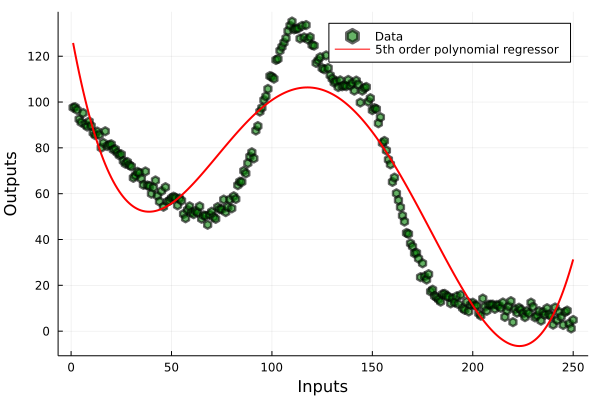
\includegraphics[clip,width=\columnwidth]{../figs/kth-poly-reg/5th-order.png}%
    }
    
    \subfloat[\centering\(K=6\)]{%
    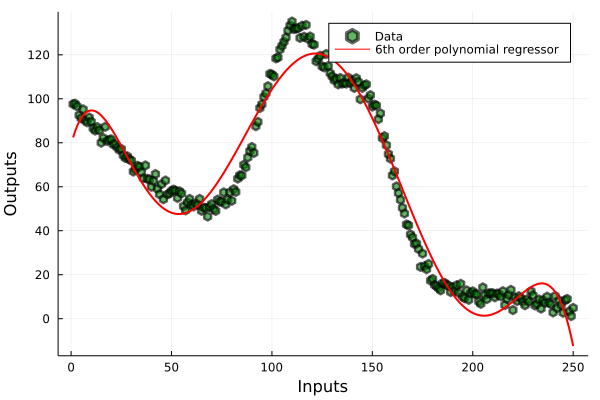
\includegraphics[clip,width=\columnwidth]{../figs/kth-poly-reg/6th-order.png}%
    \label{fig:kth-order-poly-k6}
    }

    \subfloat[\centering\(K=7\)]{%
    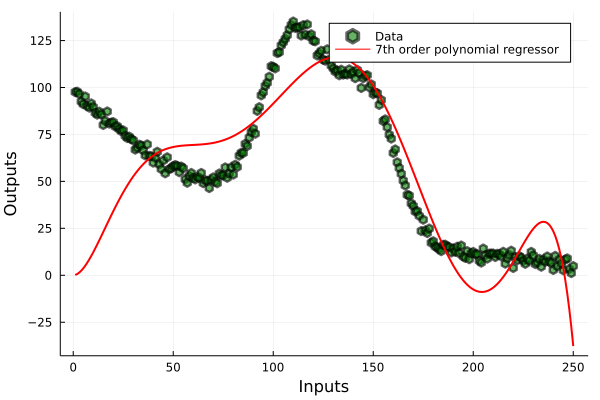
\includegraphics[clip,width=\columnwidth]{../figs/kth-poly-reg/7th-order.png}%
    \label{fig:kth-order-poly-k7}
    }
    
    \caption{The \(K\)th-order polynomial regressor.}
    \label{fig:kth-order-poly}
\end{figure}

\section{Mamdani fuzzy system}

The fuzzy system consists of a continuum-valued logic in which the truth value may be in the interval between 0 and 1. This contrasts with the so-called ordinary sets, that has only two truth values: 0 and 1. This approach enables to model the vagueness or uncertainty encountered in many real problems.

The fuzzy model maps the input variable domain to the \(\left[ 0,1 \right]\) codomain through a membership function, This process is commonly referred as fuzzification. Based on a set of rules, the fuzzy system uses the truth values of the fuzzified input to infer how much the antecedents impact the consequent. The fuzzy set obtained by the inference is then converted to a crisp value that outputs the system.

There are many different possibilities to define a fuzzy rule. A well-established fuzzy model the is the Mamdani system, which can be generically written as
\begin{align}
    &\text{IF } x_n \text{ IS } A_1 \text{ AND } x_n \text{ IS } A_2 ... \text{ AND } x_n \text{ IS } A_K \nonumber \\
    &\text{ THEN } y_n \text{ IS } B_1, \nonumber
\end{align}
where \(B_1\) and \(\left\{ A_1, A_2, \cdots, A_K \right\}\) are the output and input fuzzy sets for the \(i\)th rule, respectively, and ``AND'' is a fuzzy operator. For this problem, we consider \(K \in \left\{ 2,3 \right\}\). The set of rules applied for \(K=2\) is given by
\begin{align}
    &\text{IF } x_n \text{ IS LOW OR } x_n \text{ IS HIGH} \nonumber \\
    &\text{ THEN } y_n \text{ IS LOW}, \nonumber
\end{align}
\begin{align}
    &\text{IF } x_n \text{ IS NOT LOW AND } x_n \text{ IS NOT HIGH} \nonumber \\
    &\text{ THEN } y_n \text{ IS HIGH}, \nonumber
\end{align}
and the set of rules applied for \(K=3\) is
\begin{align}
    &\text{IF } x_n \text{ IS MEDIUM} \nonumber \\
    &\text{ THEN } y_n \text{ IS HIGH}, \nonumber
\end{align}
\begin{align}
    &\text{IF } x_n \text{ IS LOW} \nonumber \\
    &\text{ THEN } y_n \text{ IS MEDIUM}, \nonumber
\end{align}
\begin{align}
    &\text{IF } x_n \text{ IS HIGH} \nonumber \\
    &\text{ THEN } y_n \text{ IS LOW}. \nonumber
\end{align}

The fuzzy sets cited in these rules (LOW and HIGH for \(K=2\), and LOW, MEDIUM, and HIGH for \(K=3\)) are depicted in the Figure \ref{fig:input-fuzzy-sets}. The Gaussian shape of the fuzzy sets and their parameters (mean and variance) were defined experimentally in an attempt to obtain the best performance. Once the Gaussian function reaches its peak, this value it is held to maintain the true value at the extremes.
\begin{figure}[htp]
    \subfloat[\centering \(K=2\)]{%
    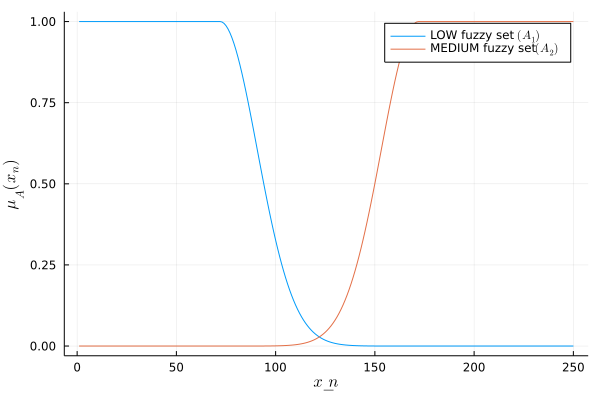
\includegraphics[clip,width=\columnwidth]{../figs/mamdani_fuzzy/fuzzification-for-2sets.png}%
    }
    
    \subfloat[\centering \(K=3\)]{%
    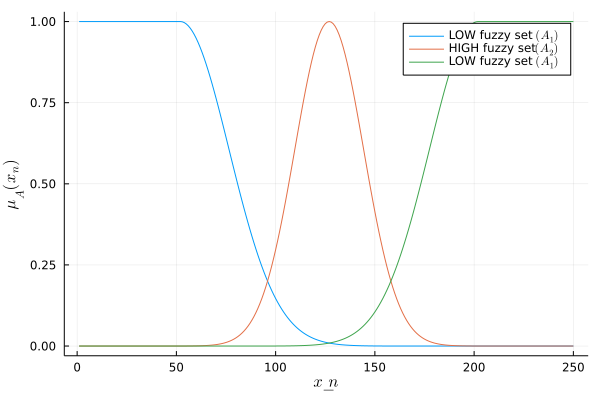
\includegraphics[clip,width=\columnwidth]{../figs/mamdani_fuzzy/fuzzification-for-3sets.png}%
    }
    
    \caption{Input fizzy sets. The output fuzzy set follows the same parameters, but with different means.}
    \label{fig:input-fuzzy-sets}
\end{figure}

After the input and output fuzzification and the rule definitions, it is necessary to define an inference method. Among the different inference methods, the Modus Ponens, defined by
\begin{align}
    \mu_{A\rightarrow B}^{(i)} (x_n;y_n) = \min\left\{  \mu_A^{(i)}(x_n), \mu_B^{(i)} (y_n) \right\},
\end{align}
is widely adopted. In this equation, \(\mu_{A\rightarrow B}^{(i)} (x_n;y_n)\) is the output fuzzy set of the \(i\)th rule and \(\mu_\cdot\) is the membership function with respect to its subscript.

The output fuzzy sets of all rules and aggregated (with the \(\vee\) operator) and the resulting fuzzy set is ``defuzzified'' to a crisp value using one of several methods described in the literature. A very popular method is the ``centroid'', which utilizes the center of mass of the output fuzzy set. The Algorithm \ref{alg:mamdani-fuzzy} summarizes the procedure of the Mamdani fuzzy system.

\begin{algorithm}[!ht]
    \DontPrintSemicolon
      
      \KwInput{\(\left\{ (x_n, y_n) \right\}_{n=1}^N\)}
    %   \KwOutput{\(\left\{ \left( \hat{a},\hat{b} \right), R^2 \right\}_{i=1}^I\)}
    %   \KwData{Testing set $x$}
    %   $\sum_{i=1}^{\infty} := 0$ \tcp*{this is a comment}
    %   \tcc{Now this is an if...else conditional loop}
    \For{\(K \in \left\{ 2,3 \right\}\)}{
        \For{\(n \in \left\{ 1, 2, \cdots, N \right\}\)}{
            \For(\tcc*[h]{for each rule}){\(i \in \left\{ 1, 2, \cdots, I \right\}\)}{
                \(\mu_{A}^{(i)}(x_n) \leftarrow\) Apply the \(i\)th rule for the set \(\left\{ \mu_{A_1}^{(i)}(x_n), \mu_{A_2}^{(i)}(x_n), \cdots, \mu_{A_K}^{(i)}(x_n) \right\}\)

                \(\mu_{A\rightarrow B}^{(i)} (x_n;y_n) \leftarrow \mu_{A}^{(i)}(x_n) \wedge \mu_{B}^{(i)}(y_n)\) \tcc{The output fuzzy set of the \(i\)th rule (Modus Ponens).}
            }

            \(\hat{y} \leftarrow \text{centroid}\left(\mu_{A\rightarrow B}^{(1)} (x_n;y_n)\right. \vee \mu_{A\rightarrow B}^{(2)} (x_n;y_n) \left. \vee \cdots \vee \mu_{A\rightarrow B}^{(I)} \right)\) \tcc{aggregation method and defuzzification}
        }
    }
    
    \caption{Mamdani fuzzy model}
    \label{alg:mamdani-fuzzy}
\end{algorithm}

The regression problem through Mamdani fuzzy system for \(K=3\) is shown in Figure \ref{fig:mamdani-fuzzy-regression}. The final model achieved a coefficient of determination of \(0.91\), and the Pearson correlation between the input and predicted value was \(0.96\).

\begin{figure}
    \centering
    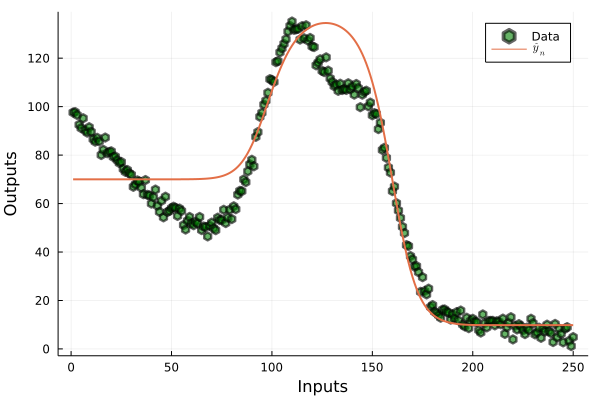
\includegraphics[scale=0.4]{../figs/mamdani_fuzzy/fuzzy_prediction.png}
    \caption{The curve fit for the Mamdani fuzzy system.}
    \label{fig:mamdani-fuzzy-regression}
\end{figure}

\bibliographystyle{bib_sobraep}
\bibliography{refs.bib}

\balance

\end{document}
